\section{Detector}

\begin{comment}
    Breve descrizione e motivazione della scelta
    Tabellina che abbiamo fatto noi
    Tabellina di Object Recognition Model Zoo
    Almeno immagine finale
\end{comment}

\begin{table}
    \centering
    \begin{tabular}{|c|c|c|c|} 
     \hline
     \textbf{Modello} & \textbf{Input size} & \textbf{Tempo} & \textbf{Prestazioni} \\
     \hline
     SSD MobileNetV1 & $640 \times 640$ & $6$ sec & Scarse \\
     \hline
     SSD ResNet152 V1 FPN & $640 \times 640$ & $20$ sec & Molto scarse \\
     \hline
     EfficientDet D3 & $896 \times 896$ & $23$ sec & Buone \\
     \hline
     Faster-RCNN ResNet101 & $1024 \times 1024$ & $20$ sec & Buone \\
     \hline
     Faster-RCNN ResNet50 & $800 \times 1333$ & $21$ sec & Ottime \\
     \hline
     Faster-RCNN ResNet101 & $800 \times 1333$ & $30$ sec & Migliori \\
     \hline
    \end{tabular}
    \caption{Confrontro tra i modelli testati. La input size è fornita in formato $h\times w$, mentre il tempo è relativo all'inferenza su una singola immagine, eseguita su una CPU virtualizzata.}
    \label{table:modelli}
\end{table}

Nello scegliere il modello abbiamo considerato come use-case di riferimento il task assegnatoci, senza calarci in una situazione di utilizzo del robot specifica (es.\@: assistenza domiciliare). Pertanto, abbiamo ritenuto necessario dare più importanza alla precisione del risultato che ai tempi di esecuzione. In un'eventuale interazione con un utente, infatti, degli errori di detection più grossolani risalterebbero maggiormente rispetto ad un tempo di attesa prolungato. Ovviamente anche quest'ultimo ha la sua importanza, visto che non ricevere feedback per un lasso di tempo prolungato potrebbe spazientire l'utente; a tal proposito, avevamo pensato che un tempo di detection\todo{direi "di attesa"} entro i 5 secondi non avrebbe creato questo problema.
Tuttavia, sull'hardware fornito per il progetto ci è impossibile tener conto del tempo di esecuzione, che risulta eccessivo con la maggior parte delle reti, anche quelle poco performanti (vedi tabella~\ref{table:modelli}). Ciò considerato, la scelta che abbiamo fatto minimizza i tempi di esecuzione tenendo però conto della precisione necessaria affinché l'interazione risulti soddisfacente.
In particolare, rispetto a quest’ultimo aspetto\todo{non si capisce bene quale sia l'aspetto} non ci è possibile fornire una valutazione quantitativa delle performance, in quanto davanti al robot si presenta sempre la stessa scena, pertanto abbiamo valutato i detector in base al loro comportamento relativamente a questa scena, e quindi i giudizi nella colonna “Performance” della tabella~\ref{table:modelli} fanno riferimento soltanto a questa condizione. Inoltre, le immagini che abbiamo catturato, a valle dello stitching, hanno una dimensione di circa $900 \times 400$. Durante le nostre prove ci siamo accorti che questo tipo di immagini non sono tipici input per le reti a nostra disposizione. Infatti alcune di queste, nonostante avessero valori di mAP di tutto rispetto sul dataset COCO \cite{modelzoo}, non risultavano efficaci nella situazione in esame.

\begin{figure}[t]
    \centering
    \hfill
    \begin{subfigure}[b]{0.49\textwidth}
        \centering
        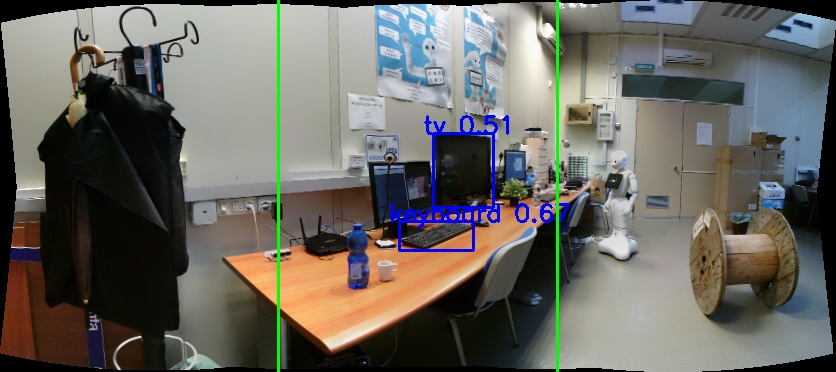
\includegraphics[width=\textwidth]{ssd_mobilenet}
        \caption{SSD MobileNetV1}
    \end{subfigure}
    \hfill
    \begin{subfigure}[b]{0.49\textwidth}
        \centering
        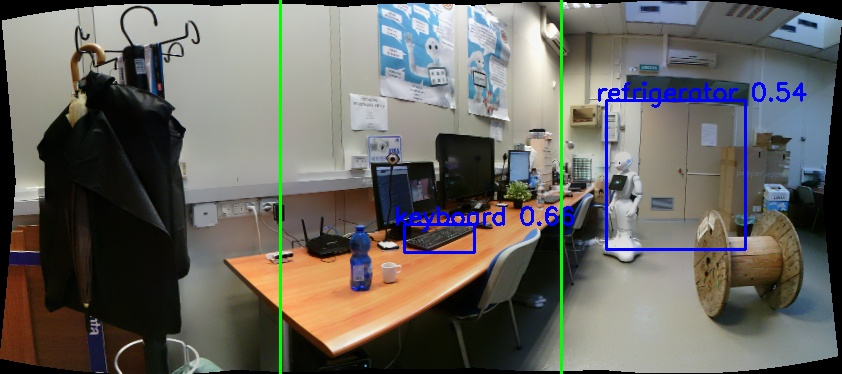
\includegraphics[width=\textwidth]{ssd_resnet152}
        \caption{SSD ResNet152}
    \end{subfigure}
    \hfill \\
    \hfill
    \begin{subfigure}[b]{0.49\textwidth}
        \centering
        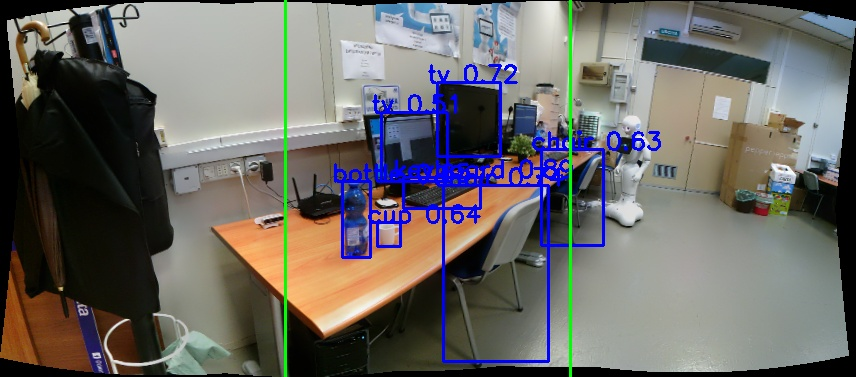
\includegraphics[width=\textwidth]{efficientdetd3}
        \caption{EfficientDet D3}
    \end{subfigure}
    \hfill
    \begin{subfigure}[b]{0.49\textwidth}
        \centering
        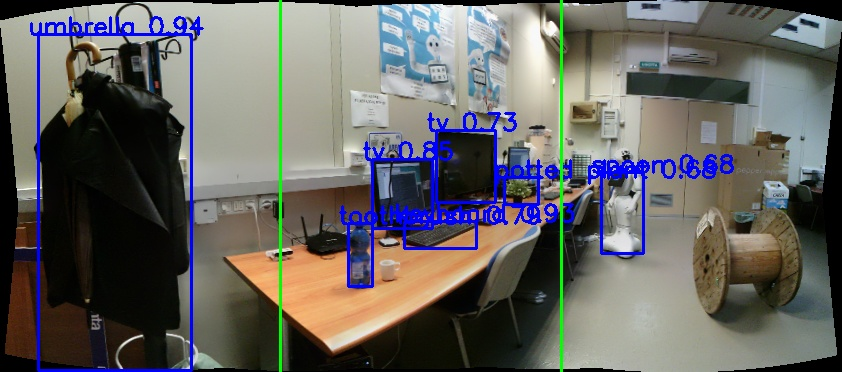
\includegraphics[width=\textwidth]{fastercnnresnet101-1024x1024.jpg}
        \caption{Faster-RCNN ResNet101 $1024\times 1024$}
    \end{subfigure}
    \hfill \\
    \hfill
    \begin{subfigure}[b]{0.49\textwidth}
        \centering
        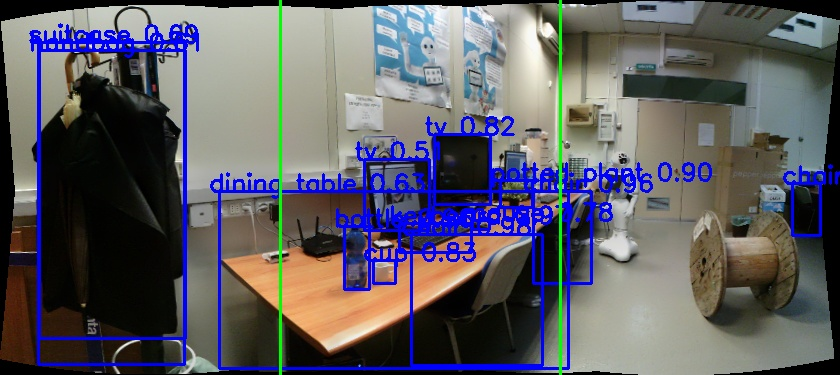
\includegraphics[width=\textwidth]{fastercnnresnet50-800x1333.jpg}
        \caption{Faster-RCNN ResNet50 $800\times 1333$}
    \end{subfigure}
    \hfill
    \begin{subfigure}[b]{0.49\textwidth}
        \centering
        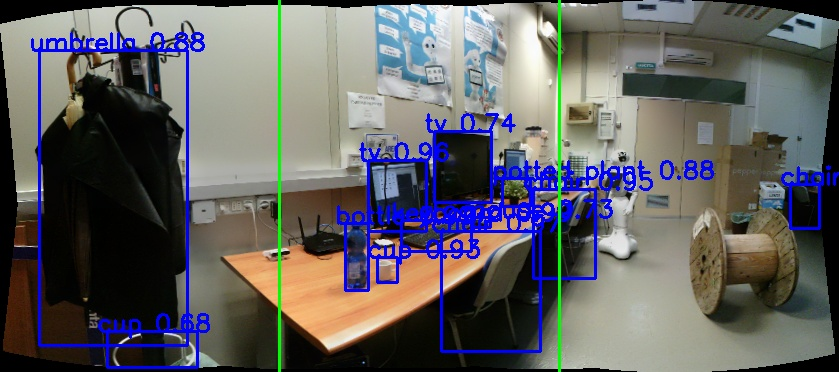
\includegraphics[width=\textwidth]{fastercnnresnet101-800x1333.jpg}
        \caption{Faster-RCNN ResNet101 $800\times 1333$}
    \end{subfigure}
    \hfill
    \caption{Risultati dei modelli testati. Le bande verticali di colore verde fluo evidenziano la suddivisione dell’immagine utilizzata per separare tra loro le regioni sinistra, destra e centrale.}
\end{figure}

Inizialmente sono state provate due reti che lavorano con immagini aventi risoluzione $640 \times 640$ che, però, facendo un downscale della panoramica data in input, hanno dimostrato pessime performance.
Abbiamo quindi deciso di provare reti che lavorano con immagini aventi una risoluzione più grande. Faster-RCNN che usa come backbone ResNet101 con input size $1024 \times 1204$, avendo performance discrete nella detection (non tutti gli oggetti venivano rivelati ed ad altri veniva assegnata l’etichetta sbagliata), ha dimostrato che la risoluzione delle immagini in input deve essere un altro fattore discriminante nella scelta del modello.

Il passo successivo è stato provare una rete che lavorasse con immagini più simili, in risoluzione, a quelle che noi le forniamo in input: Faster-RCNN con backbone ResNet50 e input size $800 \times 1333$ ha dimostrato, in tempi simili alle altre reti, ottime performance in termini di rilevazione degli oggetti, ma a qualche oggetto veniva assegnata una label sbagliata; Faster-RCNN con backbone ResNet101 e input size $800 \times 1333$ ha dimostrato le migliori performance sia per la classificazione che per la detection, ma in tempi più dilatati, pertanto abbiamo preferito tenere come nostro modello di riferimento Faster-RCNN basata su ResNet50. I dati sui confronti tra questi modelli sono riportati in tabella~\ref{table:modelli}. Nello scegliere questa rete abiamo anche tenuto conto delle prestazioni riportate nella tabella \cite{modelzoo}, ed in particolare, per il detector selezionato, queste sono tali per cui, se anche dovesse essere eseguito su hardware che ne incrementi il tempo di esecuzione di un ordine di grandezza, la detection richiederebbe comunque meno dei 5 secondi che ci eravamo prefissati come limite.

Faster-RCNN consiste di una \emph{Region Proposal Network} (RPN) e una rete\todo{aggiungerei "neurale convoluzionale"} che si occupa della classificazione, ed entrambe condividono le feature convoluzionali\todo{scriverei "feature map dei livelli convoluzionali"} dell'intera immagine. Le feature maps estratte dai layer convoluzionali sono date in input alla RPN, la quale utilizza una sliding window, e per ogni finestra genera $k$ anchor boxes di diverse forme e grandezze aventi centro coincidente con quello della finestra \cite{frcnn}. La backbone ResNet50 è un'architettura basata su ResNet con 50 livelli, la quale sfrutta il principio del \emph{residual learning} per ottenere una rete abbastanza profonda che non sia affetta dal problema del \emph{vanishing gradient} e che sia meno complessa di altre reti della letteratura \cite{resnet}. Nel confronto con altre architetture, Faster-RCNN risulta essere la migliore per la detection di oggetti di medie e piccole dimensioni \cite{speedaccuracy}, che sono quelli principalmente presenti nelle nostre immagini (vedi paragrafo~\ref{sec:master_small_img}).

